\subsection*{Equation de diffusion}
\begin{equation*}
    u_t=ku_{xx}
\end{equation*}
\textbf{Principe du maximum:}\\
Si u(x, t) satisfait l'équation de diffusion dans un rectangle
(disons, $0 \leq x \leq l$, $0 \leq t \leq T$) dans l'espace-temps, alors la valeur
maximale de $u(x, t)$ est atteinte soit initialement ($t = 0$), soit sur
les côtés ($x = 0$ ou $x = l$)
\begin{figure}[H]
    \centering
    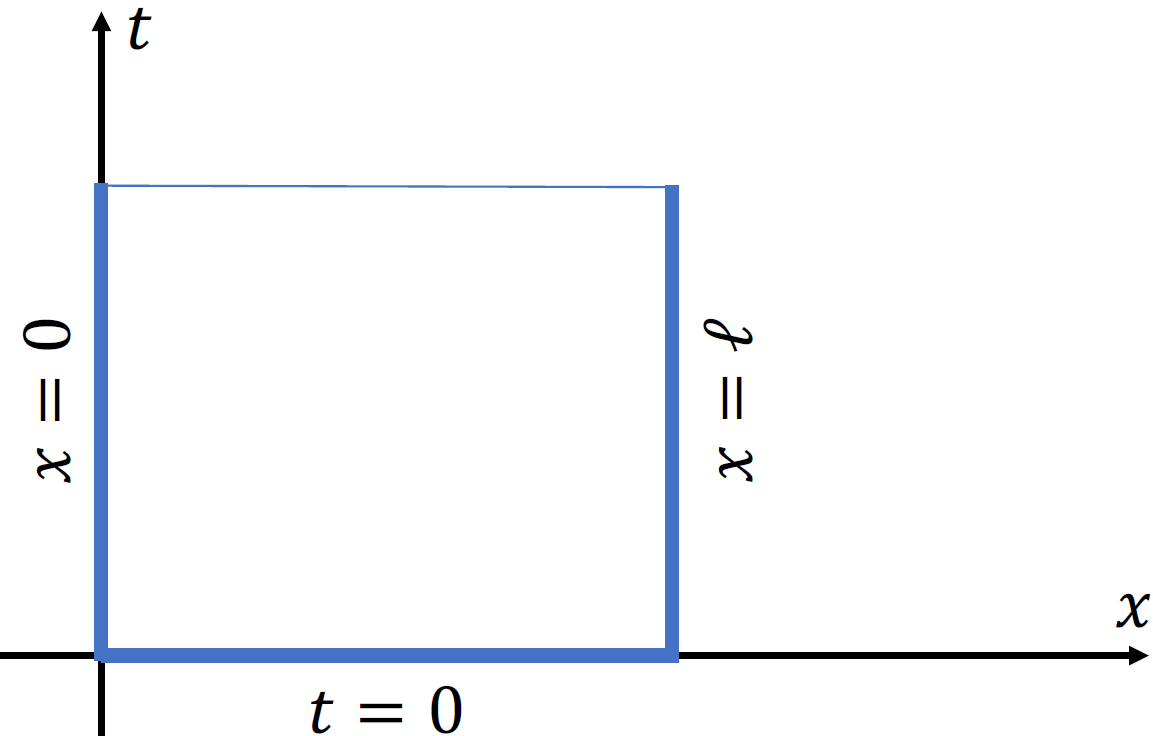
\includegraphics[width=0.5\linewidth]{images/semaine3_principe_max.png}
\end{figure}
La valeur minimale à la même propriété.\\
\textbf{Solution avec condition initiale:}
\begin{equation*}
    \boxed{u(x,t)=\frac{1}{2\sqrt{\pi kt}}\int_{-\infty}^{+\infty}e^{-\frac{(x-y)^2}{4kt}}\phi(y)\mathrm{d}y}
\end{equation*}
\textbf{Fonction d'erreur:}
\begin{subequations}
    \begin{equation*}
        \text{erf}(x)=\frac{2}{\sqrt{\pi}}\int_0^xe^{-p^2}\mathrm{d}p
    \end{equation*}
    \begin{equation*}
        \left\{
        \begin{aligned}
             & \int_{-\infty}^{\infty}e^{-p^2}\mathrm{d}p=\sqrt{\pi} \\
             & \int_{0}^{\infty}e^{-p^2}\mathrm{d}p=\frac{1}{2}
        \end{aligned}
        \right.
    \end{equation*}
\end{subequations}
Résoudre l'équation de diffusion avec la condition initiale:
\begin{equation*}
    \left\{
    \begin{aligned}
         & \phi(x)=1\quad\text{pour}\quad x>0 \\
         & \phi(x)=3\quad\text{pour}\quad x<0
    \end{aligned}
    \right.
\end{equation*}
\begin{figure}[H]
    \centering
    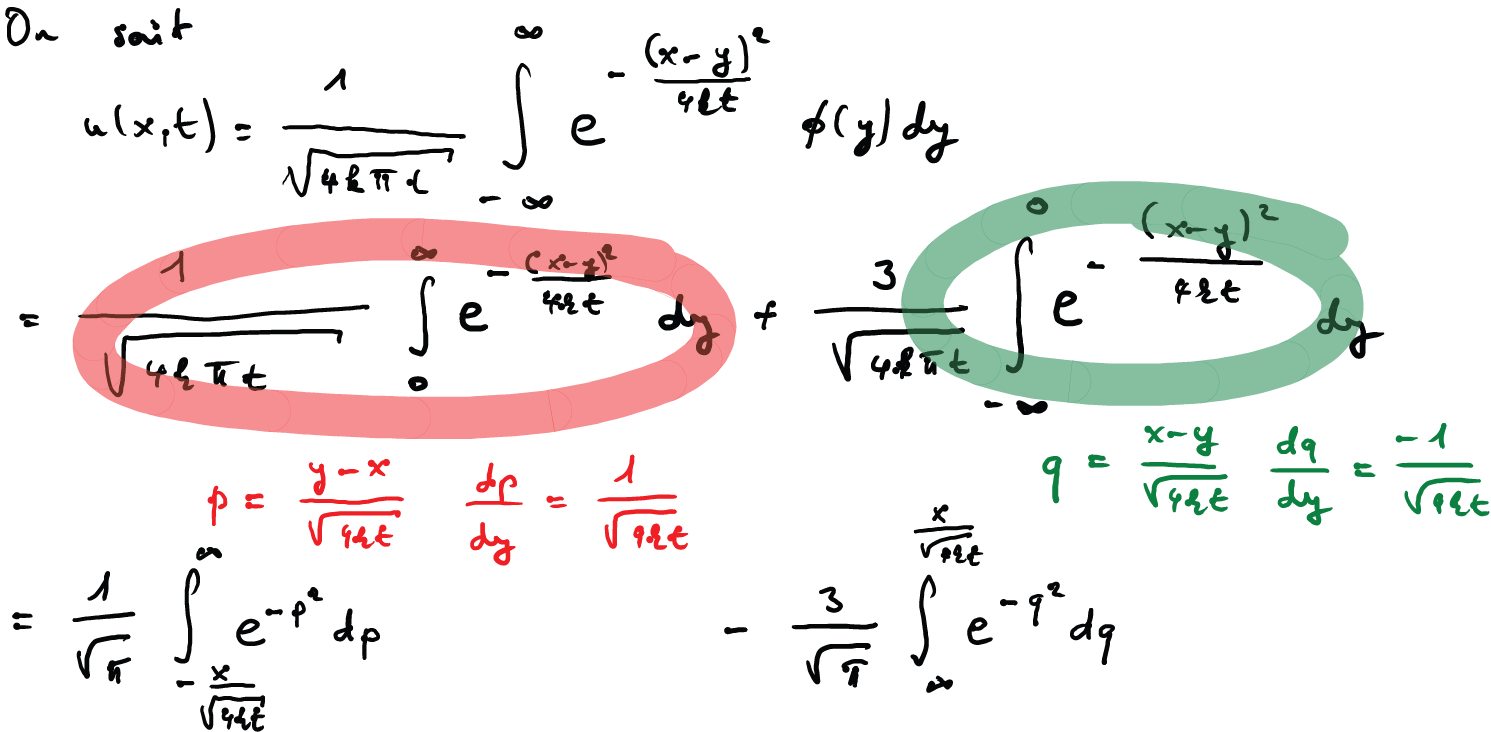
\includegraphics[width=\linewidth]{images/semaine3_diff1.png}
\end{figure}
\begin{figure}[H]
    \centering
    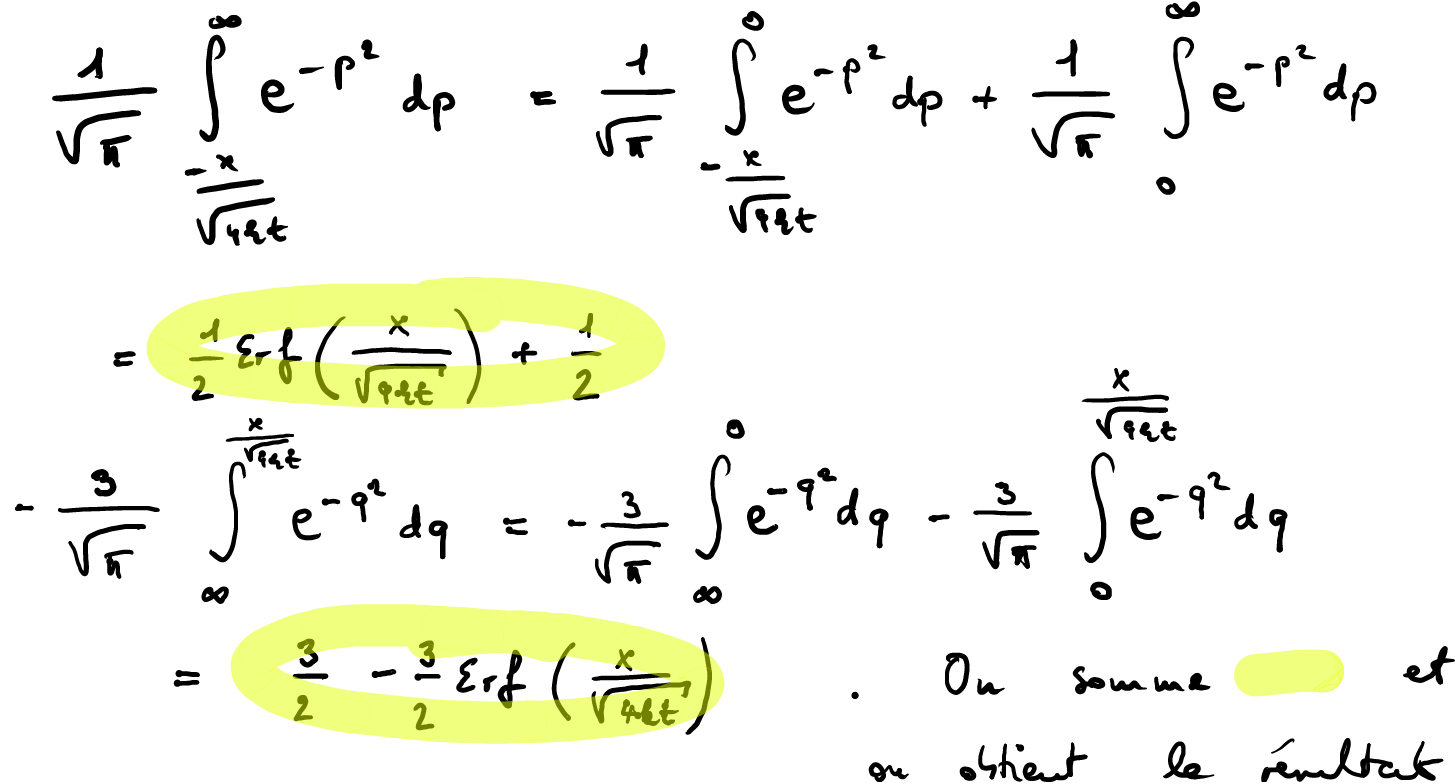
\includegraphics[width=\linewidth]{images/semaine3_diff2.png}
\end{figure}


